
%
% File sem_syn_diff.tex


\documentclass[11pt,letterpaper]{article}
\usepackage[letterpaper]{geometry}
\usepackage{acl2012}
\usepackage{times}
\usepackage{latexsym}
\usepackage{amsmath}
\usepackage{multirow}
\usepackage{url}
\usepackage{tikz}
\usepackage{tikz-dependency}
\usepackage[warn]{textcomp}
\usepackage[font=small]{caption}
\usepackage{subcaption}
\usepackage{multirow}
\usepackage{etoolbox}
\usepackage{xr}
\usepackage{listings}

\makeatletter
\newcommand{\@BIBLABEL}{\@emptybiblabel}
\newcommand{\@emptybiblabel}[1]{}
\makeatother
\usepackage[hidelinks]{hyperref}
\DeclareMathOperator*{\argmax}{arg\,max}

\newcommand{\com}[1]{}
\newcommand{\oa}[1]{\footnote{\color{red}OA: #1}}
\newcommand{\daniel}[1]{\footnote{\color{blue}Daniel: #1}}

\hyphenation{SemEval}


\lstset{basicstyle=\ttfamily}


\usetikzlibrary{shapes,shapes.misc}

%\aclfinalcopy % Uncomment this line for the final submission
\def\aclpaperid{***}

%\setlength\titlebox{5cm}
% You can expand the titlebox if you need extra space
% to show all the authors. Please do not make the titlebox
% smaller than 5cm (the original size); we will check this
% in the camera-ready version and ask you to change it back.

\title{Why Semantics is Harder than Syntax}

\author{First Author \\
  Affiliation / Address line 1 \\
  Affiliation / Address line 2 \\
  Affiliation / Address line 3 \\
  {\tt email@domain} \\\And
  Second Author \\
  Affiliation / Address line 1 \\
  Affiliation / Address line 2 \\
  Affiliation / Address line 3 \\
  {\tt email@domain} \\}

\date{}

\begin{document}

\maketitle

\begin{abstract}
To explain the difference in scores between syntactic and semantic parsers,
we explore the various factors and perform experiments to demonstrate them.
As a test case, we take Universal Dependencies (UD) and
Universal Conceptual Cognitive Annotation (UCCA).
By creating a full conversion protocol, we develop a novel UCCA parser.
\end{abstract}

\section{Introduction}\label{sec:introduction}

Semantic representation schemes have seen major progress in recent years.
In parallel, syntactic representation is becoming more semantic.
However, looking at the absolute scores achieved in semantic parsing tasks
as opposed to syntactic parsing,
there is still a gap:
UCCA parsers get just about 75\% F-score, whereas UD parsers get more than 85\% LAS F1. Why?
UD has much more training data (UCCA: 5K, UD: about 17K for English).
But inter-annotator agreement is also lower: about 85\% for UCCA, and more than 95\% for UD.

Several questions naturally manifest themselves:
how much of the difference is explained by the differences in---
\begin{itemize}
\item Evaluation metric,
\item Amount of training data,
\item Maturity of technology dedicated to the scheme,
\item Learnability of the scheme.
\end{itemize}

Learnability, in turn, is affected by
\begin{itemize}
\item Formal annotation choices \cite{Schwartz:12},
\item Actual content that the scheme attempts to capture.
\end{itemize}


The gap can be bridged by fine-grained semantic annotation,
such as adposition and case supersenses
\cite{schneider2017adposition,blodgett2018semantic}.

To explore the difference in content, we experiment with converting UD to UCCA
using a multi-step protocol:
\begin{enumerate}
\item Augment UD trees to get \textit{enhanced++} dependencies \cite{SCHUSTER16.779}, hence UD$^{++}$.
\item Structurally convert bilexical dependency graphs into constituency-like graphs by inserting
  non-terminal nodes and \textit{head} edges (\S\ref{sec:conversion}).
\item Translate UD relations into UCCA edge labels,
  either by a deterministic mapping (\S\ref{sec:mapping})
  or through learning (\S\ref{sec:learning}).
\end{enumerate}

%%%%%%%%%%%%%%%%%%%%%%%%%%%%%%%%%%%%%%%%%%%%%%%%%%%%%%%%%%%%%%%%%%%%%%%%%%%%%%%%%
\section{Related Work}\label{sec:related_work}

\paragraph{AMR parsing.}

\newcite{wang2015transition,wang-xue-pradhan:2015:ACL-IJCNLP,wang-EtAl:2016:SemEval,goodman2016noise,wang2017getting}
presented a transition-based AMR parser, CAMR, which requires a
syntactic dependency tree as input.
It operates on the input tree, transforming it into an AMR graph
by a sequence of transitions.
The accuracy of the underlying syntactic dependency parser is important,
as shown by \newcite{wang-xue-pradhan:2015:ACL-IJCNLP},
who achieved the best results using the Charniak parser trained on a
much larger and more diverse dataset---the full OntoNotes corpus,
rather than the Stanford parser trained on the Penn TreeBank.

\newcite{szubert2018structured} showed that when comparing AMR to Universal Dependencies (UD),
97\% of AMR edges are evoked by words or syntactic relations.


%%%%%%%%%%%%%%%%%%%%%%%%%%%%%%%%%%%%%%%%%%%%%%%%%%%%%%%%%%%%%%%%%%%%%%%%%%%%%%%%%

\section{Representations}\label{sec:representations}

\paragraph{Universal Conceptual Cognitive Annotation.}\label{sec:ucca}
UCCA \cite{abend2013universal} is a semantic representation whose main design principles
are ease of annotation, cross-linguistic applicability, and a modular architecture.
UCCA represents the semantics of linguistic utterances
as directed acyclic graphs (DAGs), where terminal (childless) nodes
correspond to the text tokens, and non-terminal nodes to semantic units that participate
in some super-ordinate relation.
Edges are labeled, indicating the role of a child in the relation the parent represents.
Nodes and edges belong to one of several \textit{layers}, each corresponding
to a ``module'' of semantic distinctions.
UCCA's \textit{foundational layer} (the only layer for which annotated data exists)
mostly covers predicate-argument structure, semantic heads and inter-Scene relations.

UCCA distinguishes \textit{primary} edges, corresponding 
to explicit relations, from \textit{remote} edges (appear dashed in
Figure~\ref{fig:example_ucca}) that allow for a unit to participate
in several super-ordinate relations.
Primary edges form a tree in each layer, whereas remote edges enable reentrancy, forming a DAG.


\begin{figure}[!ht]
  \centering
    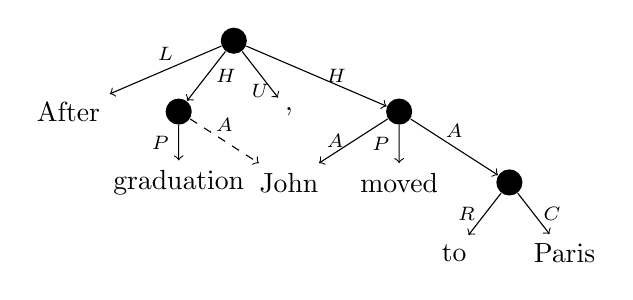
\begin{tikzpicture}[level distance=9mm, sibling distance=14mm, ->,
        every circle node/.append style={fill=black}]
      \tikzstyle{word} = [font=\rmfamily,color=black]
      \node (ROOT) [circle] {}
        child {node (After) [word] {After} edge from parent node[above] {\scriptsize $L$}}
        child {node (graduation) [circle] {}
        {
          child {node [word] {graduation} edge from parent node[left] {\scriptsize $P$}}
        } edge from parent node[right] {\scriptsize $H$} }
        child {node [word] {,} edge from parent node[below] {\scriptsize $U$}}
        child {node (moved) [circle] {}
        {
          child {node (John) [word] {John} edge from parent node[left] {\scriptsize $A$}}
          child {node [word] {moved} edge from parent node[left] {\scriptsize $P$}}
          child {node [circle] {}
          {
            child {node [word] {to} edge from parent node[left] {\scriptsize $R$}}
            child {node [word] {Paris} edge from parent node[right] {\scriptsize $C$}}
          } edge from parent node[above] {\scriptsize $A$} }
        } edge from parent node[right] {\scriptsize $H$} }
        ;
      \draw[dashed,->] (graduation) to node [above] {\scriptsize $A$} (John);
    \end{tikzpicture}
\caption{\label{fig:example_ucca}
 Example UCCA graph. The dashed edge is remote.
  Pre-terminal nodes and edges are omitted for brevity.}
\end{figure}

%%%%%%%%%%%%%%%%%%%%%%%%%%%%%%%%%%%%%%%%%%%%%%%%%%%%%%%%%%%%%%%%
\paragraph{Universal Dependencies.}\label{sec:ud}
UD \cite{nivre2016universal,11234/1-2515} has quickly become
the dominant dependency scheme for
syntactic  annotation in many languages,
aiming for cross-linguistically consistent and coarse-grained treebank
annotation. Formally, UD uses bilexical trees, with edge labels 
representing syntactic relations between words.
Figure~\ref{fig:original_example_ud} shows an example UD tree.

We use UD as an auxiliary task,
inspired by previous work on joint syntactic and semantic parsing
(see \S\ref{sec:related_work}).
In order to reach comparable analyses cross-linguistically,
UD often ends up in annotation that is similar to the common practice
in semantic treebanks, such as linking content words to content words wherever possible.
Using UD further allows conducting experiments on languages other than English, 
for which AMR and SDP annotated data is not available (\S\ref{sec:experiments}).

In addition to basic UD trees, we use the \textit{enhanced++} UD graphs available for English,
which are generated by the Stanford CoreNLP converters \cite{SCHUSTER16.779}.
These include additional and augmented relations between content words,
partially overlapping with the notion of remote edges in UCCA:
in the case of control verbs, for example, a direct relation is added in 
enhanced++ UD between the subordinated verb and its controller,
which is similar to the semantic schemes' treatment of this construction.

\begin{figure}[!ht]

\fbox{\begin{subfigure}{0.47\textwidth}
  \centering
    \begin{dependency}[text only label, label style={above}, font=\small]
    \begin{deptext}[column sep=.8em,ampersand replacement=\^]
    After \^ graduation \^ , \^ John \^ moved \^ to \^ Paris \\
    \end{deptext}
        \depedge[edge unit distance=1ex]{2}{1}{case}
        \depedge[edge unit distance=1ex]{4}{3}{punct}
        \depedge[edge unit distance=1ex]{5}{4}{nsubj}
        \depedge[edge unit distance=1ex, edge end x offset=-2pt]{2}{5}{obl}
        \depedge[edge unit distance=1ex]{7}{6}{case}
        \deproot[edge unit distance=1.5ex]{5}{root}
        \depedge[edge unit distance=1.5ex]{5}{7}{obl}
    \end{dependency}
  \caption{UD \label{fig:original_example_ud}}
\end{subfigure}}

\fbox{\begin{subfigure}{0.47\textwidth}
  \centering
  \scalebox{.95}{
  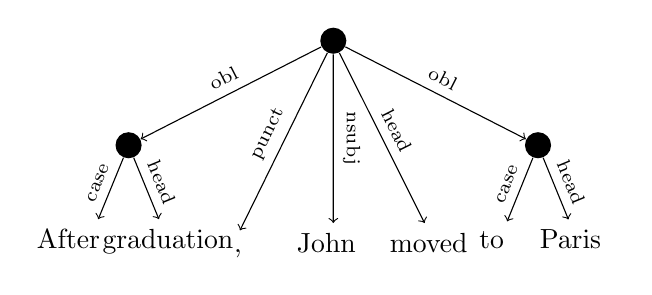
\begin{tikzpicture}[level distance=15mm, ->,
      every node/.append style={sloped,anchor=south,auto=false,font=\scriptsize},
      level 1/.style={sibling distance=13mm},
      level 2/.style={sibling distance=1cm}]
    \tikzstyle{word} = [font=\rmfamily,color=black]
    \node (ROOT) [fill=black,circle] {}
      child {node (after) [fill=black,circle] {}
      {
        child {node [word] {After{\color{white}g}\quad\quad} edge from parent node {case}}
        child {node [word] {\quad graduation\quad\quad} edge from parent node {head}}
      } edge from parent node {obl}}
      child {node {}
      {
        child {node [word] (comma) {\quad,{\color{white}g}} edge from parent [draw=none]}
      } edge from parent [draw=none]}
      child {node {}
      {
        child {node [word] (John) {John{\color{white}g}} edge from parent [draw=none]}
      } edge from parent [draw=none]}
      child {node {}
      {
        child {node [word] (moved) {moved{\color{white}g}} edge from parent [draw=none]}
      } edge from parent [draw=none]}
      child {node (to) [fill=black,circle] {}
      {
          child {node [word] {to{\color{white}g}} edge from parent node {case}}
          child {node [word] {Paris{\color{white}g}} edge from parent node {head}}
      } edge from parent node {obl}}
      ;
      \draw (ROOT) to node {punct} (comma);
      \draw (ROOT) to node {nsubj} (John);
      \draw (ROOT) to node {head} (moved);
  \end{tikzpicture}}
  \captionof{figure}{UD}\label{fig:converted_example_ud}
\end{subfigure}}

\caption{Figure \ref{fig:original_example_ud} presents a UD tree.
  Edge labels express syntactic relations.
Figure~\ref{fig:converted_example_ud} presents a converted UD graph
(with pre-terminals omitted: each terminal drawn in place of its parent).
Intermediate non-terminals and \textit{head} edges are introduced.
While converted UD graphs form trees, enhanced++ UD graphs may not.}\label{fig:ud_examples}
\end{figure}


\section{Amount of training data}\label{sec:data_size}


\begin{table*}[t]
\centering
\small
\setlength\tabcolsep{2pt}
\begin{tabular}{l|ccc|ccc||ccc|ccc||ccc|ccc}
& \multicolumn{6}{c||}{\footnotesize \bf English}
& \multicolumn{6}{c||}{\footnotesize \bf French}
& \multicolumn{6}{c}{\footnotesize \bf German} \\
\hline
& \multicolumn{3}{c|}{\footnotesize \bf {\#} tokens}
& \multicolumn{3}{c||}{\footnotesize \bf {\#} sentences}
& \multicolumn{3}{c|}{\footnotesize \bf {\#} tokens}
& \multicolumn{3}{c||}{\footnotesize \bf {\#} sentences}
& \multicolumn{3}{c|}{\footnotesize \bf {\#} tokens}
& \multicolumn{3}{c}{\footnotesize \bf {\#} sentences} \\
& \footnotesize \bf train & \footnotesize \bf dev & \footnotesize \bf test
& \footnotesize \bf train & \footnotesize \bf dev & \footnotesize \bf test
& \footnotesize \bf train & \footnotesize \bf dev & \footnotesize \bf test 
& \footnotesize \bf train & \footnotesize \bf dev & \footnotesize \bf test
& \footnotesize \bf train & \footnotesize \bf dev & \footnotesize \bf test
& \footnotesize \bf train & \footnotesize \bf dev & \footnotesize \bf test \\
\hline
\textbf{UCCA} &&&&&&&&&&&&&&&& \\
Wiki & 128444 & 14676 & 15313 & 4268 & 454 & 503 &&&&&&&&&&&& \\
20K &&& 12339 &&& 506 & 10047 & 1558 & 1324 & 413 & 67 & 67 & 79894 & 10059 & 42366 & 3429 & 561 & 2164 \\
\textbf{UD} & \multicolumn{2}{l}{458277} && \multicolumn{2}{l}{17062} &&
\multicolumn{2}{l}{899163} && \multicolumn{2}{l}{32347} && \multicolumn{2}{l}{268145} && 13814
\end{tabular}
\caption{Number of tokens and sentences in the training, development and test sets
we use for each corpus and language.\label{tab:corpora}}
\end{table*}

Syntactic dependency parsers require many training examples to achieve
state-of-the-art results.
Even after around 500K tokens, the learning curves do not seem to saturate
\cite{de2017old,velldal2017joint}.

Whereas the largest UCCA training set (English Wiki) contains 128K tokens,
The joined English UD training sets contain 458K tokens.
In French UCCA has just 10K training tokens whereas UD has 899K,
and in German UCCA has 80K and UD 268K.

\begin{table}[t]
\centering
\begin{tabular}{l|lll|lll}
& \multicolumn{3}{c|}{\footnotesize \bf Primary} & \multicolumn{3}{c}{\footnotesize \bf Remote} \\
& \footnotesize \textbf{LP} & \footnotesize \textbf{LR} & \footnotesize \textbf{LF}
& \footnotesize \textbf{LP} & \footnotesize \textbf{LR} & \footnotesize \textbf{LF} \\
\hline
\footnotesize 10\% \\
\footnotesize 20\% \\
\footnotesize 30\% \\
\footnotesize 40\% \\
\footnotesize 50\% \\
\footnotesize 60\% \\
\footnotesize 70\% \\
\footnotesize 80\% \\
\footnotesize 90\% \\
\footnotesize 100\% \\
\end{tabular}
\caption{
Results for TUPA \protect\cite{hershcovich2017a} when trained on increasing amount of training data
(English Wiki corpus).
\label{tab:partial_data_results}}
\end{table}

Table~\ref{tab:partial_data_results} shows results for TUPA,
trained on 10\%, 20\% etc. of the Wiki training set and tested on the Wiki test set.


\section{Structural Conversion}\label{sec:conversion}

To parse text into UD, we use UDPipe \cite{udpipe:2017}.
On UD v1.2, UDPipe achieved 80.2\% LAS $F_1$ on English using automatic POS tags.
On French it achieved 77.8\% and on German 71.8\%.

We extend the conversion protocol by \newcite{hershcovich2018multitask},
converting UD into a unified DAG format.
The format consists of a rooted DAG, where the tokens are the terminal nodes.
As in the UCCA format, edges are labeled (but not nodes),
and are divided into \textit{primary} and \textit{remote} edges,
where the primary edges form a tree (all nodes have at most one primary parent,
and the root has none).
Remote edges enable reentrancy, and thus together with primary edges
form a DAG.
Figure~\ref{fig:converted_example_ud} shows an example for a converted graph.

To convert UD into the unified DAG format,
we add a pre-terminal for each token,
and attach the pre-terminals according to the original dependency edges:
traversing the tree from the root down, for each head token we create a non-terminal
parent with the edge label {\it head},
and add the node's dependents as children of the created non-terminal node.
In case of reentrancy, an arbitrary parent is marked as primary, and the rest as remote
(denoted as dashed edges in Figure~\ref{fig:converted_example_ud}).

Table~\ref{tab:conversion_results_unlabeled} shows unlabeled evaluation of the
structurally converted UD graphs as compared to gold-annotated UCCA graphs.


\begin{table}[t]
\centering
\begin{tabular}{l|lll|lll}
& \multicolumn{3}{c|}{\footnotesize \bf Primary} & \multicolumn{3}{c}{\footnotesize \bf Remote} \\
& \footnotesize \textbf{UP} & \footnotesize \textbf{UR} & \footnotesize \textbf{UF}
& \footnotesize \textbf{UP} & \footnotesize \textbf{UR} & \footnotesize \textbf{UF} \\
\hline
\multicolumn{4}{l|}{\small \bf WSJ (manually annotated)} & \\
\footnotesize UD
& 85.2 & 88.5 & 86.8 & -- & 0 & 0 \\
\footnotesize UD$^{++}$
& 82.7 & 85.9 & 84.3 & 12.5 & 12.7 & 12.6 \\
\footnotesize TUPA
& 84.3 & 84.2 & 84.3 & 39.5 & 30.9 & 34.7 \\
\\
\multicolumn{4}{l|}{\small \bf WSJ (automatically parsed)} & \\
UDPipe & 81.5 & 84.5 & 83 & -- & 0 & 0 \\
\footnotesize TUPA
& 83.9 & 83.7 & 83.8 & 40.5 & 30.9 & 35.1
\end{tabular}
\caption{
Unlabeled precision, recall and $F_1$ (in~\%) for primary and remote edges.
For comparison, TUPA \protect\cite{hershcovich2017a} is trained on Wikipedia with features predicted by UDPipe
and tested on WSJ with gold POS and dependency features (above)
or on WSJ with gold POS and dependency features (below).
\label{tab:conversion_results_unlabeled}}
\end{table}


\section{Deterministic label mapping}\label{sec:mapping}


Using the standard UCCA evaluation
script,\footnote{\url{http://github.com/danielhers/ucca/blob/master/scripts/evaluate_standard.py}}
we created a confusion matrix between the edge tags in converted UD trees
and the annotated UCCA graphs (see Table~\ref{tab:confusion_matrix}).
Edges are matched by terminal yield.
In this confusion matrix, we can see what is the most common UCCA edge label corresponding
to each UD relation.
To convert the UD graphs into fully labeled UCCA graphs,
we replace each UD edge label with its most common UCCA counterpart.

The \textit{head} edges introduced as part of the conversion do not have a single
corresponding UCCA edge label---although C (center) is the most common corresponding label,
other labels such as P (process) are also common.
This is a difference between UD, which selects the most central token to be the head of a phrase,
to UCCA, which also annotates the relation between that head and the unit it is part of.
To overcome this limitation, we replace all \textit{head} labels with C, but then
apply standard UCCA normalization to the resulting graphs after conversion,
replacing C with P when it has sibling A's (participants) or
with H when it has sibling H's (parallel scenes).
We select P rather than S (state) as the main relation in the normalization because
it is much more common (14,719 P's in the Wiki corpus as opposed to 3354 S's).

\begin{table}[t]
\centering
\begin{tabular}{ll|r}
UD & UCCA & count \\
\hline
head & C & 508 \\
case & R & 231 \\
det & E & 196 \\ 
amod & E & 129 \\
compound & E & 113 \\
head & P & 109 \\
nsubj & A & 106 \\
dobj & A & 51 \\
nummod & E & 33 \\
cc & N & 32 \\
advmod & D & 31 \\
conj:and & C & 26
\end{tabular}
\caption{Excerpt from UD-UCCA confusion matrix calculated from the WSJ dataset.
Each row shows the number of times an edge was labeled with a specific label in UD
and another specific label in UCCA.\label{tab:confusion_matrix}}
\end{table}

\paragraph{Conversion of gold UD annotations.}

We performed this conversion on the 100 human-annotated UD sentences
and evaluated on the human-annotated UCCA graphs on the same sentences.
The results appear in Table~\ref{tab:conversion_results_labeled}.

\begin{table}[t]
\centering
\begin{tabular}{l|lll|lll}
& \multicolumn{3}{c|}{\footnotesize \bf Primary} & \multicolumn{3}{c}{\footnotesize \bf Remote} \\
& \footnotesize \textbf{LP} & \footnotesize \textbf{LR} & \footnotesize \textbf{LF}
& \footnotesize \textbf{LP} & \footnotesize \textbf{LR} & \footnotesize \textbf{LF} \\
\hline
\multicolumn{4}{l|}{\small \bf WSJ (manually annotated)} & \\
\footnotesize UD
& 68.3 & 71 & 69.6 & -- & 0 & 0 \\
\footnotesize UD$^{++}$
& 66.3 & 68.9 & 67.6 & 10.7 & 10.9 & 10.8 \\
\footnotesize TUPA
& 69.7 & 69.6 & 69.7 & 39.5 & 30.9 & 34.7 \\
\\
\multicolumn{4}{l|}{\small \bf WSJ (automatically parsed)} & \\
UDPipe & 63.3 & 65.7 & 64.5 & -- & 0 & 0 \\
\footnotesize TUPA
& 69.6 & 69.4 & 69.5 & 40.5 & 30.9 & 35.1
\end{tabular}
\caption{
Labeled precision, recall and $F_1$ (in~\%) for primary and remote edges,
of passages converted automatically from UD to UCCA,
with mapped edge labels, as evaluated against gold UCCA.
For comparison, TUPA \protect\cite{hershcovich2017a} is trained on Wikipedia with features predicted by UDPipe
and tested on WSJ with gold POS and dependency features (above)
or on WSJ with POS and dependency features predicted by UDPipe (below).
\label{tab:conversion_results_labeled}}
\end{table}

Despite the simple conversion protocol, labeled scores are quite high.
For comparison, the unlabeled evaluation (Table~\ref{tab:conversion_results_unlabeled})
servers as an oracle experiment for the labeled conversion,
and is an upper bound given a fixed structural conversion.

\paragraph{Conversion of automatically parsed UD annotations.}

To be able to evaluate the conversion on a larger corpus,
such as the UCCA Wiki set, which does not have UD annotations,
we use an automatic UD parser: UDPipe.
The results appear in Table~\ref{tab:conversion_results_labeled}.


\section{Learned label reassignment}\label{sec:learning}

Rather than mapping syntactic UD labels to semantic UCCA labels
by a fixed set of replacements, we can use the context to learn
which replacement to apply, closing the gap between the labeled
and unlabeled scores.


\section{Analysis of differences}\label{sec:analysis}



As an example for divergence between the schemes, Figure~\ref{fig:wsj_0011.8} shows
the same sentence after conversion and as manually annotated.
This short sentence got an $F_1$ of 34.8\%.


\begin{figure*}[!ht]
\fbox{\begin{subfigure}{\textwidth}
\begin{dependency}
\begin{deptext}[column sep=2em]
% sent_id = wsj_0011.8
% text = Imports were at $ 50.38 billion , up 19 % .
% doc_id = wsj_0011
Imports \& were \& at  \& \$   \& 50.38 \& billion \& ,     \& up  \& 19  \& \%   \& .    \\
%NOUN    \& AUX  \& ADP \& SYM \& NUM   \& NUM     \& PUNCT \& ADV \& NUM \& SYM \& PUNCT \\
\end{deptext}
\depedge{4}{1}{nsubj}
\depedge{4}{2}{cop}
\depedge{4}{3}{case}
\deproot{4}{root}
\depedge{6}{5}{compound}
\depedge{4}{6}{nummod}
\depedge{4}{7}{punct}
\depedge{4}{8}{advmod}
\depedge{10}{9}{nummod}
\depedge{8}{10}{obl:npmod}
\depedge{4}{11}{punct}
\end{dependency}
\caption{Original UD tree.\label{fig:wsj_0011.8_ud}}
\end{subfigure}}
\fbox{\begin{subfigure}{\textwidth}
  \centering
  \scalebox{.95}{
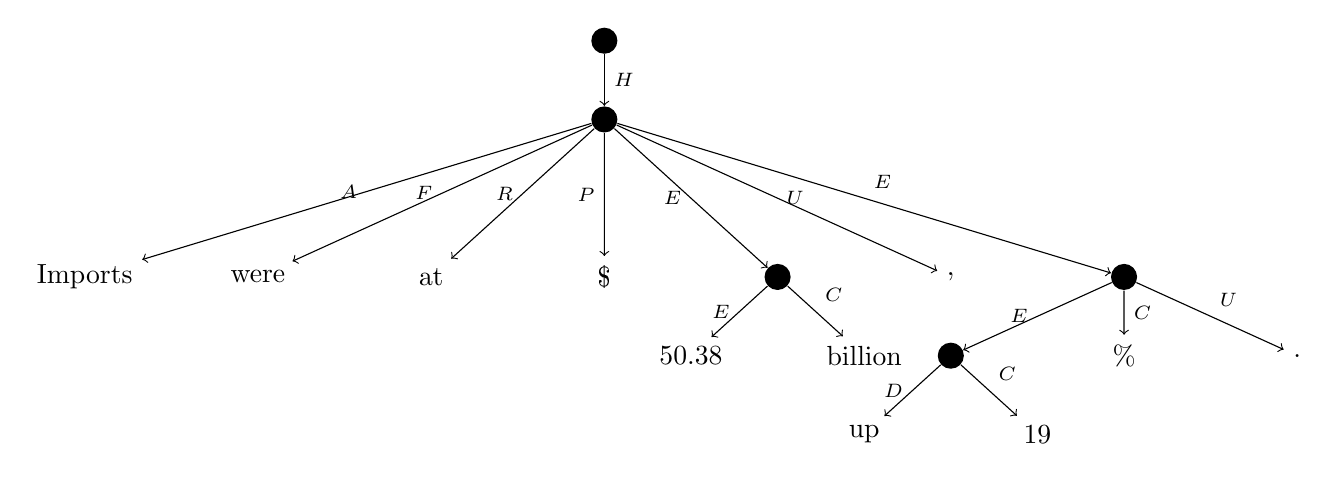
\begin{tikzpicture}[->,level distance=1cm, sibling distance=22mm,
  level 2/.style={level distance=2cm,
  level 3/.style={level distance=1cm}},
  every circle node/.append style={fill=black}]
  \tikzstyle{word} = [font=\rmfamily,color=black]
  \node (1_1) [circle] {}
  {
  child {node (1_2) [circle] {}
    {
    child {node (1_4) [word] {Imports}  edge from parent node[left]  {\scriptsize $A$}}
    child {node (1_5) [word] {were}  edge from parent node[left]  {\scriptsize $F$}}
    child {node (1_6) [word] {at}  edge from parent node[left]  {\scriptsize $R$}}
    child {node (1_3) [word] {\$}  edge from parent node[left]  {\scriptsize $P$}}
    child {node (1_7) [circle] {}
      {
      child {node (1_13) [word] {50.38}  edge from parent node[left]  {\scriptsize $E$}}
      child {node (1_8) [word] {billion}  edge from parent node[auto]  {\scriptsize $C$}}
      } edge from parent node[left]  {\scriptsize $E$}}
    child {node (1_9) [word] {,}  edge from parent node[right]  {\scriptsize $U$}}
    child {node (1_10) [circle] {}
      {
      child {node (1_14) [circle] {}
        {
        child {node (1_16) [word] {up}  edge from parent node[left]  {\scriptsize $D$}}
        child {node (1_15) [word] {19}  edge from parent node[auto]  {\scriptsize $C$}}
        } edge from parent node[left]  {\scriptsize $E$}}
      child {node (1_11) [word] {\%}  edge from parent node[auto]  {\scriptsize $C$}}
      child {node (1_12) [word] {.}  edge from parent node[auto]  {\scriptsize $U$}}
      } edge from parent node[auto]  {\scriptsize $E$}}
    } edge from parent node[auto]  {\scriptsize $H$}}
  }
;
\end{tikzpicture}
  }\caption{Converted from gold UD to UCCA.\label{fig:wsj_0011.8_converted}}
\end{subfigure}}
  
\fbox{\begin{subfigure}{\textwidth}
  \centering
  \scalebox{.95}{
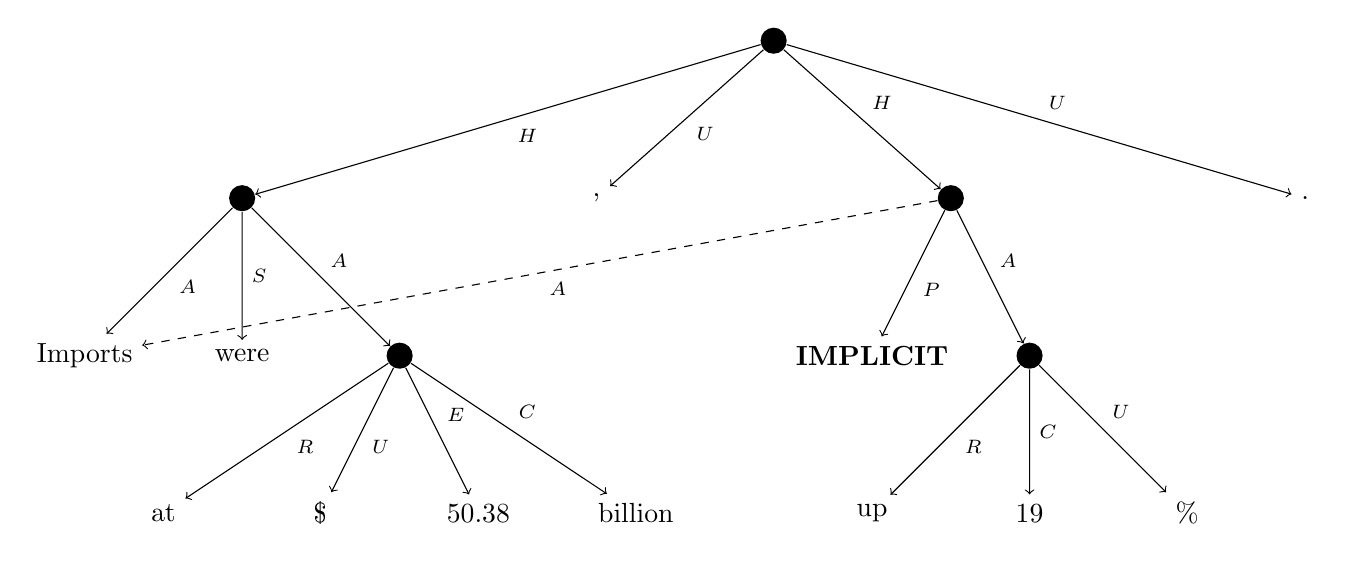
\begin{tikzpicture}[->,level distance=2cm,
  level 1/.style={sibling distance=45mm},
  level 2/.style={sibling distance=2cm},
  level 3/.style={sibling distance=2cm},
  every circle node/.append style={fill=black}]
  \tikzstyle{word} = [font=\rmfamily,color=black]
  \node (1_1) [circle] {}
  {
  child {node (1_2) [circle] {}
    {
    child {node (1_3) [word] {Imports}  edge from parent node[auto]  {\scriptsize $A$}}
    child {node (1_4) [word] {were}  edge from parent node[auto]  {\scriptsize $S$}}
    child {node (1_5) [circle] {}
      {
      child {node (1_6) [word] {at}  edge from parent node[auto]  {\scriptsize $R$}}
      child {node (1_14) [word] {\$}  edge from parent node[auto]  {\scriptsize $U$}}
      child {node (1_8) [word] {50.38}  edge from parent node[auto]  {\scriptsize $E$}}
      child {node (1_9) [word] {billion}  edge from parent node[auto]  {\scriptsize $C$}}
      } edge from parent node[auto]  {\scriptsize $A$}}
    } edge from parent node[auto]  {\scriptsize $H$}}
  child {node (1_15) [word] {,}  edge from parent node[auto]  {\scriptsize $U$}}
  child {node (1_10) [circle] {}
    {
    child {node (1_18) [word] {\textbf{IMPLICIT}}  edge from parent node[auto]  {\scriptsize $P$}}
    child {node (1_11) [circle] {}
      {
      child {node (1_12) [word] {up}  edge from parent node[auto]  {\scriptsize $R$}}
      child {node (1_13) [word] {19}  edge from parent node[auto]  {\scriptsize $C$}}
      child {node (1_16) [word] {\%}  edge from parent node[auto]  {\scriptsize $U$}}
      } edge from parent node[auto]  {\scriptsize $A$}}
    } edge from parent node[auto]  {\scriptsize $H$}}
  child {node (1_17) [word] {.}  edge from parent node[auto]  {\scriptsize $U$}}
  };
  \draw[dashed,->] (1_10) to node [auto] {\scriptsize $A$} (1_3);
\end{tikzpicture}
  }\caption{Manually annotated UCCA.\label{fig:wsj_0011.8_orig}}
  
\end{subfigure}}

\caption{UCCA graphs for sentence \lstinline{wsj_0011.8}\label{fig:wsj_0011.8}}

\end{figure*}

More differences:
\begin{itemize}
\item Identity vs. set membership in copular constructions:
    ``Mr. Vinken is chairman of Elsevier N.V.'' vs. ``The morbidity rate is a striking finding''.
\item Infinitive vs. purpose ``to''. 
\end{itemize}


\section{Experiments}\label{sec:experiments}

\begin{table*}[t]
\centering
\small
\setlength\tabcolsep{2pt}
\begin{tabular}{l|ccc|ccc||ccc|ccc||ccc|ccc}
& \multicolumn{6}{c||}{\footnotesize \bf English}
& \multicolumn{6}{c||}{\footnotesize \bf French}
& \multicolumn{6}{c}{\footnotesize \bf German} \\
\hline
& \multicolumn{3}{c|}{\footnotesize \bf {\#} tokens}
& \multicolumn{3}{c||}{\footnotesize \bf {\#} sentences}
& \multicolumn{3}{c|}{\footnotesize \bf {\#} tokens}
& \multicolumn{3}{c||}{\footnotesize \bf {\#} sentences}
& \multicolumn{3}{c|}{\footnotesize \bf {\#} tokens}
& \multicolumn{3}{c}{\footnotesize \bf {\#} sentences} \\
& \footnotesize \bf train & \footnotesize \bf dev & \footnotesize \bf test
& \footnotesize \bf train & \footnotesize \bf dev & \footnotesize \bf test
& \footnotesize \bf train & \footnotesize \bf dev & \footnotesize \bf test 
& \footnotesize \bf train & \footnotesize \bf dev & \footnotesize \bf test
& \footnotesize \bf train & \footnotesize \bf dev & \footnotesize \bf test
& \footnotesize \bf train & \footnotesize \bf dev & \footnotesize \bf test \\
\hline
Wiki & 128444 & 14676 & 15313 & 4268 & 454 & 503 &&&&&&&&&&&& \\
20K &&& 12339 &&& 506 & 10047 & 1558 & 1324 & 413 & 67 & 67 & 79894 & 10059 & 42366 & 3429 & 561 & 2164
\end{tabular}
\caption{Number of tokens and sentences in the training, development and test sets
we use for each corpus and language.\label{tab:corpora}}
\end{table*}

\paragraph{Data.}

For UCCA, we use v1.2 of the English Wikipedia corpus \cite{abend2013universal},
with the standard train/dev/test split (see Table~\ref{tab:corpora}),
and the \textit{Twenty Thousand Leagues Under the Sea} corpora
\cite{sulem2015conceptual},
annotated in English, French and German.\footnote{\url{http://github.com/UniversalConceptualCognitiveAnnotation}}
%For English and French we use 20K v1.0,
%a small parallel corpus comprising the first five chapters of the book.
%As in previous work \cite{hershcovich2017a}, we use the English part only as an out-of-domain test set.
%We train and test on the French part using the standard split,
%as well as the German corpus (v0.9),
%which is a pre-release and still contains a considerable amount of noisy annotation.

We also use 100 English sentences from Section 02 of the Penn Treebank Wall Street Journal
(PTB WSJ),
annotated by a single expert UCCA annotator \cite{hershcovich2018multitask},
and publicly available.\footnote{\url{http://github.com/UniversalConceptualCognitiveAnnotation/UCCA_English-WSJ}}
These sentences had already been annotated by the PTB scheme.
We convert the PTB format to UD$^{++}$ v1 using Stanford CoreNLP,
to UD v2 using Udapi\footnote{\url{http://github.com/udapi/udapi-python}},
and then to the unified DAG format using our protocol.


\begin{table}[t]
\centering
\small
\setlength\tabcolsep{3pt}
\begin{tabular}{l|lll|lll}
& \multicolumn{3}{c|}{\footnotesize \bf Primary} & \multicolumn{3}{c}{\footnotesize \bf Remote} \\
& \footnotesize \textbf{LP} & \footnotesize \textbf{LR} & \footnotesize \textbf{LF}
& \footnotesize \textbf{LP} & \footnotesize \textbf{LR} & \footnotesize \textbf{LF} \\
\hline
\multicolumn{4}{l|}{\small \bf English (Wiki, in-domain)} & \\
\footnotesize HAR18 Single
& 74.4 & 72.9 & 73.6 & 53 & 50 & 51.5 \\
\footnotesize HAR18 MTL UD$^{++}$
& 75 & 73.2 & 74.1 & 49 & 52.7 & 50.8 \\
\footnotesize Converted UD aux.
\\
\hline\\
\multicolumn{4}{l|}{\small \bf English (20K, out-of-domain)} & \\
\footnotesize HAR18 Single
& 69 & 69 & 69 & 41.2 & 19.8 & 26.7 \\
\footnotesize HAR18 MTL UD$^{++}$
& 69.6 & 69.8 & 69.7 & 41.4 & 22 & 28.7 \\
\footnotesize Converted UD aux.
\\
\hline\\
\multicolumn{4}{l|}{\small \bf French (20K, in-domain)} & \\
\small HAR18 Single & 68.2 & 67 & 67.6 & 26 & \enskip 9.4 & 13.9 \\
\small HAR18 MTL UD & 70.3 & 70 & 70.1 & 43.8 & 13.2 & 20.3 \\
\footnotesize Converted UD aux.
\\
\hline\\
\multicolumn{4}{l|}{\small \bf German (20K, in-domain)} & \\
\small HAR18 Single & 73.3 & 71.7 & 72.5 & 57.1 & 17.7 & 27.1 \\
\small HAR18 MTL UD & 73.7 & 72.6 & 73.2 & 61.8 & 24.9 & 35.5 \\
\footnotesize Converted UD aux.
\\
\end{tabular}
\caption{
Labeled precision, recall and $F_1$ (in~\%) for primary and remote edges,
on the Wiki and 20K test sets.
HAR18: \protect\newcite{hershcovich2018multitask}.}\label{tab:aux_results}
\end{table}

\paragraph{Using converted UD as auxiliary data.}

\newcite{hershcovich2018multitask} used UD as an auxiliary task for UCCA parsing,
treating UD parsing as an auxiliary task and using a multitask learning model
with hard parameter sharing.
We perform a similar experiment, but instead of a multitask model,
we use UD data converted to UCCA and train on it with the same single-task model.
Table~\ref{tab:aux_results} shows the results of this experiment.

\paragraph{Fine-grained evaluation of UCCA parsing performance.}

\newcite{damonte-17,szubert2018structured} suggested fine-grained evaluation measures
for AMR parsing, using sub-tasks of the AMR parsing task or UD labels to evaluate on.
Similarly, our conversion protocol allows fine-grained evaluation of UCCA parsing.
Table~\ref{tab:fine_grained_ucca} shows fine-grained evaluation according to UCCA categories, and
Table~\ref{tab:fine_grained_ud} shows fine-grained evaluation according to UD relations.


\begin{table}[t]
\centering
\small
\setlength\tabcolsep{3pt}
\begin{tabular}{l|l}
nsubj & 0.92 \\ 
Terminal & 1.0 \\ 
head & 0.999 \\ 
cop & 1.0 \\ 
det & 1.0 \\    
compound & 0.995 \\ 
amod & 0.974 \\ 
case & 0.994 \\ 
obj & 0.808 \\ 
aux & 1.0 \\ 
cc & 0.98 \\ 
conj & 0.769 \\ 
advmod & 0.95 \\ 
mark & 1.0 \\ 
nmod & 0.606 \\ 
obl & 0.623 \\ 
appos & 0.571 \\ 
nummod & 0.865 \\ 
acl & 0.486 \\ 
advcl & 0.696 \\ 
xcomp & 0.636 \\ 
iobj & 0.8 \\ 
ccomp & 0.571 \\ 
fixed & 1.0 \\ 
dep & 0.737 \\ 
expl & 1.0 \\  
parataxis & 1.0
\end{tabular}
\caption{
Fine-grained labeled $F_1$ according to UCCA categories,
of TUPA trained on Wiki with features extraced by UDPipe
and evaluated on WSJ with features extraced by UDPipe.}
\label{tab:fine_grained_ucca}
\end{table}

\begin{table}[t]
\centering
\small
\setlength\tabcolsep{3pt}
\begin{tabular}{l|l}
ParallelScene & 0.539 \\ 
Function & 0.705 \\ 
Participant & 0.578 \\ 
Punctuation & 0.98 \\ 
Process & 0.699 \\ 
State & 0.289 \\ 
Elaborator & 0.686 \\ 
Center & 0.757 \\ 
Terminal & 1.0 \\ 
Relator & 0.85 \\ 
Connector & 0.778 \\ 
Adverbial & 0.541 \\ 
Linker & 0.658 \\ 
Ground & 0.0
\end{tabular}
\caption{
Fine-grained labeled $F_1$ according to gold UD relations,
of TUPA trained on Wiki with features extraced by UDPipe
and evaluated on WSJ with features extraced by UDPipe.}
\label{tab:fine_grained_ud}
\end{table}


%\paragraph{Experimental setup.}
%
%
%\paragraph{Evaluation.}
%
%
%
%\section{Results}\label{sec:results}
%
%\section{Discussion}\label{sec:discussion}
%
%
%\section{Conclusion}\label{sec:conclusion}


\bibliography{references}
\bibliographystyle{acl2012}

\end{document}
